\section{Data}
\label{sec:data}

\subsection{\Glsfmtfullpl{gemm}}
\label{sec:mouse_models}
\glsunset{gemm}
Mouse models play a crucial role in breast cancer research, offering a powerful
tool for understanding the molecular mechanisms of disease development and
progression.
\Glspl{gemm} allow researchers to manipulate specific genes, such as those
involved in estrogen signaling\supercite{park_mouse_2018}.
These models can closely mimic human breast cancer, providing insights into the
initiation, progression, and metastasis of tumors in a controlled and
reproducible environment\supercite{pfefferle_transcriptomic_2013}.
Additionally, mouse models enable the study of cancer within the context of a
living organism, allowing for the evaluation of hormonal influences, immune
responses, and interactions with the tumor
microenvironment\supercite{manning_mouse_2016}.
This makes them indispensable for preclinical testing of new therapies,
including hormone-targeting treatments like \gls{tam} and aromatase inhibitors,
which are standard in the management of \gls{hr+} breast
cancer\supercite{fan_endocrine_2015,yin_disruption_2014}.
By studying cancer in mice, researchers can identify potential biomarkers,
refine therapeutic strategies, and deepen our understanding of the pathways
driving breast cancer in humans\supercite{peterson_amphiregulin_2015}.

\subsection{Datasets}
\label{sec:datasets}
The datasets used in this thesis are derived from two complementary studies by
\textcite{furth_esr1_2023,furth_overexpression_2023} that investigate the role
of estrogen signaling in breast cancer through the use of \glspl{gemm}.

One dataset comes from an aging study, which focuses on how the overexpression
of \gls{esr1} and \gls{cyp19} in mammary epithelial cells influences cancer
development as the mice age past reproductive senescence.
Details about these genes can be found in \cref{sec:important_genes}.
The second dataset originates from an anti-hormonal study, which examines the
effects of \gls{tam} and \gls{let} treatments on \glspl{gemm} during
reproductive senescence.
Both treatment agents have been described in \cref{sec:important_treatments}.

Both datasets provide critical insights into the molecular mechanisms linking
aging, estrogen signaling, and breast cancer progression.

\subsubsection{Study design}

In both studies, the \glspl{gemm} were modified to overexpress either
\gls{esr1} or \gls{cyp19} in their mammary epithelial cells when treated with
doxycycline.
This genetic manipulation was designed to model increased estrogen signaling,
which is known to be a critical factor in breast cancer development, especially
after menopause\supercite{furth_esr1_2023,furth_overexpression_2023}.
The studies focused on inducing this overexpression at or around reproductive
senescence, which is a model for menopause in women, to better understand the
increased cancer risks in aging mammary
tissue\supercite{furth_esr1_2023,furth_overexpression_2023}.

The timeline of the two studies is illustrated in \cref{fig:dataset_timeline}.

\begin{figure}[ht]
    \centering

    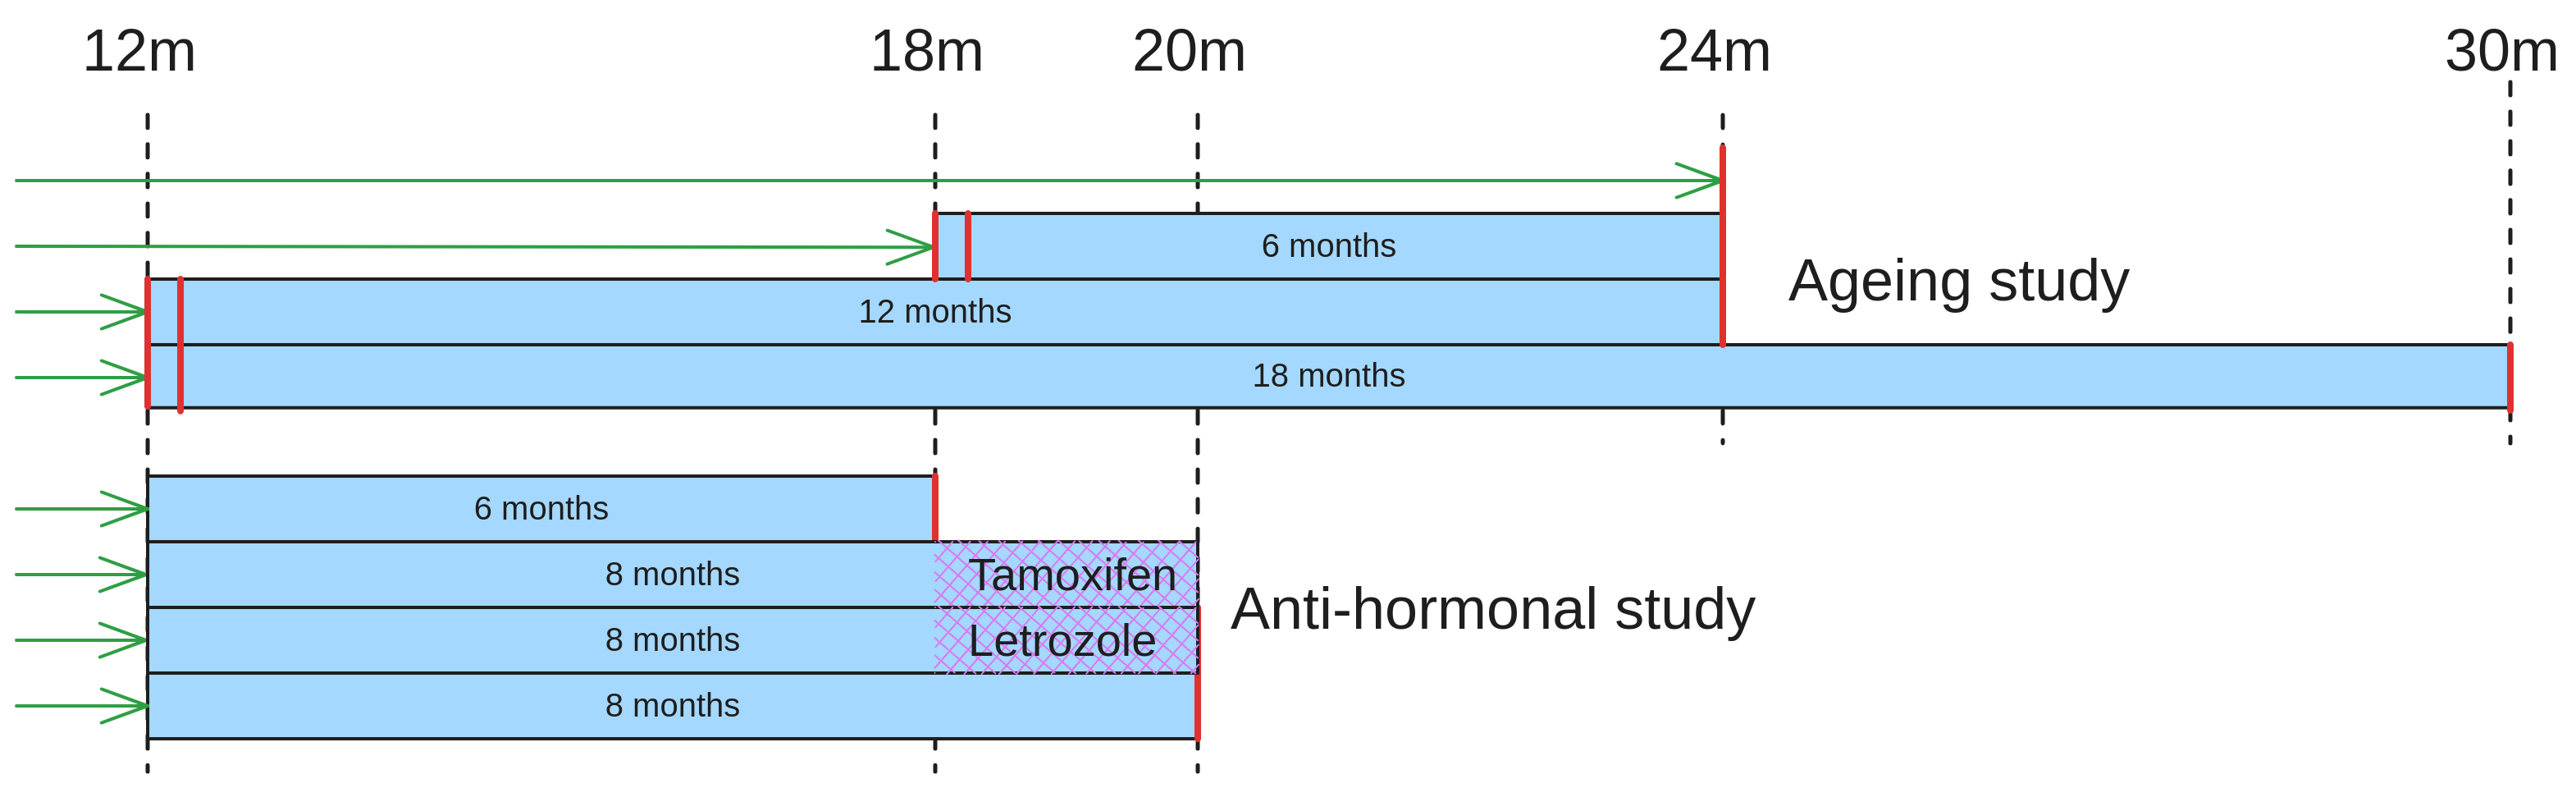
\includegraphics[width=\textwidth]{chapters/3_materials_and_methods/figures/datasets.png}
    \caption{Overview of the two studies and their respective timelines.
        Each red line represents two cohorts of mice that were euthanized for tissue
        collection: one with the \gls{esr1} transgene and one with the \gls{cyp19}
        transgene.
        The green arrows indicate periods without transgene induction, while the blue
        blocks indicate the periods of doxycycline treatment to induce the transgenes.
    } \label{fig:dataset_timeline} \end{figure}

\subsubsection{Differences in treatment}
The key difference between the two studies lies in the timing and duration of
the transgene induction, as well as the subsequent treatment with anti-hormonal
therapies.

\paragraph{Anti-hormonal study}
In the anti-hormonal study, eight different cohorts of mice were investigated,
four with the \gls{esr1} transgene and four with the \gls{cyp19} transgene.
As shown in \cref{fig:dataset_timeline}, the mice were treated with doxycycline
to induce the transgenes at 12 months of age, corresponding to middle age in
humans.

At 18 months of age (6 months of transgene induction), one cohort of each
genotype was euthanized to collect mammary gland tissue as a pre-treatment
control.
At the same time, two cohorts of each genotype were started being treated with
\gls{tam} or \gls{let}, respectively.
The remaining cohort of each genotype was left untreated as a control.

After two more months (now 20 months of age), the remaining three cohorts
(\gls{tam}, \gls{let}, control) of each genotype were
euthanized\supercite{furth_esr1_2023}.

\paragraph{Aging study}
The aging study consists of 16 cohorts of mice, eight with the \gls{esr1}
transgene and eight with the \gls{cyp19} transgene.
At 12 months of age, one cohort of each genotype was euthanized to collect
mammary gland tissue as a pre-transgene induction control.
For three cohorts of each genotype, the transgene induction was started at 12
months of age.

One of the three cohorts with transgene induction started at 12 months was
euthanized after 1 week of doxycycline treatment to assess the immediate
effects of the transgene induction.
The remaining two cohorts were euthanized at 24 and 30 months of age to
investigate the long-term effects of the transgene induction.

One cohort of each genotype that did not receive the transgene induction was
euthanized at 18 months of age.
Two other cohorts of each genotype started the transgene induction at 18 months
of age.
Of these two cohorts, one was euthanized after 1 week of doxycycline treatment,
while the other was euthanized at 24 months of age.

Lastly, one cohort of each genotype that did not receive any transgene
induction was euthanized at 24 months of
age\supercite{furth_overexpression_2023}.

\subsubsection{Sequencing process} \label{sec:dataset_sequencing}
Both studies used \gls{rna-seq} to analyze gene expression in the mammary
glands.
After euthanasia, thoracic mammary glands were flash frozen, and \gls{rna} was
extracted using a Direct Zol \gls{rna} miniprep kit.
The sequencing libraries were prepared from ribosome-depleted \gls{rna} and
sequenced using the Illumina NextSeq 550 platform with a single-end 75-bp read
length\supercite{furth_esr1_2023,furth_overexpression_2023}.

\subsubsection{Findings}

\paragraph{Anti-hormonal study}
The study found that \gls{esr1} overexpression significantly increased the
expression of genes related to cell proliferation, particularly those linked to
poor prognostic indicators in early-stage \gls{hr+} breast cancer.
\Gls{tam} and \gls{let} treatments were able to reduce this elevated
proliferative signature, but only \gls{esr1} mice showed substantial
responsiveness to \gls{tam} during reproductive senescence.
Both models were responsive to \gls{let} before and after reproductive
senescence\supercite{furth_esr1_2023}.

\paragraph{Aging study}
This study demonstrated that \gls{esr1} overexpression in aged mice led to a
higher prevalence of \gls{er+} mammary adenocarcinomas.
The tumors in \gls{esr1}-overexpressing mice were predominantly \gls{er+},
whereas \gls{cyp19} mice exhibited a mix of \gls{er+} and adenosquamous
carcinomas.
The \gls{esr1} mice developed a persistent proliferative signature similar to
that found in human \gls{er+} breast cancer, supporting the role of aging and
prolonged estrogen exposure in the generation of these
cancers\supercite{furth_overexpression_2023}.

\subsection{\Glsfmtshort{mirna} data}
\label{sec:mirna_data}

As explained in \cref{sec:circrna_mirna_sponging}, \gls{mirna} sponging is one
of the most well-known functions of \glspl{crna}.
Unfortunately, the datasets described in \cref{sec:datasets} do not include
\gls{mirna} data - thus, it is not possible to identify \glspl{mirna} that were
actually present in the mice.

The closest alternative is using information from other studies that
investigated the \gls{mirna} expression in the same tissue and under similar
conditions.
For this purpose, I found a study by \textcite{wang_dynamic_2022} that
investigates how \glspl{mirna} are involved in regulating milk protein gene
expression during different stages of mammary gland development in mice.
The following paragraphs provide an overview of the study design and the main
findings.

\subsubsection{Study design}
The study collected mammary gland tissues from 15 specific-pathogen-free (SPF)
female ICR mice across five developmental stages: virgin, day 16 of pregnancy,
day 12 of lactation, and days 1 and 3 of forced weaning.
Tissues were frozen for RNA extraction, and small \glspl{rna} ranging from 18
to 30 nucleotides were isolated.
Adapter ligation and cDNA synthesis were performed, followed by amplification
for sequencing.
Using the DNBseq platform, approximately 21 million clean reads were generated
per sample.
After filtering low-quality reads, the clean reads were mapped to the mouse
genome with Bowtie2, identifying known \glspl{mirna} from existing databases,
while novel \glspl{mirna} were predicted using miRDeep2.
These miRNAs were grouped into 12 clusters based on expression profiles across
the developmental stages using the Mfuzz R package, revealing stage-specific
patterns.
Validation of the sequencing data was performed by qPCR on eight randomly
selected \glspl{mirna}, with strong correlation to the sequencing results.
Target genes of the \glspl{mirna} were predicted using TargetScan, miRanda, and
RNAhybrid, and functional analysis through \gls{go} and \gls{kegg} pathway
analysis revealed their involvement in mammary gland development and
lactation\supercite{wang_dynamic_2022}.

\subsubsection{Findings}
The study uncovered several key findings regarding the role of \glspl{mirna} in
regulating mammary gland development and milk protein expression in mice.
Researchers identified a total of 852 known \glspl{mirna} and 179 novel
\glspl{mirna} in the mammary glands across five investigated developmental
stages.
These \glspl{mirna} were grouped into 12 clusters based on their expression
patterns, with Cluster 1 \glspl{mirna} showing an inverse relationship with
milk protein gene expression.
Notably, the study identified a novel \gls{mirna}, mmu-miR424-5p, which was
found to regulate the expression of CSN2 (\textbeta{}-casein), a key milk
protein gene, indicating its role as a potential negative regulator of milk
protein synthesis\supercite{wang_dynamic_2022}.

The functional analysis of these \glspl{mirna} revealed that their target genes
were involved in crucial biological processes related to mammary gland
development, such as cell proliferation, differentiation, apoptosis, and lipid
metabolism.
Pathway analyses (\gls{go} and \gls{kegg}) further linked these \glspl{mirna}
to important signaling pathways, including the Wnt, mTOR, and MAPK pathways,
which are known to regulate mammary gland growth, differentiation, and milk
production\supercite{wang_dynamic_2022}.
